% ------------------------------------------------------------------------ %
% !TEX encoding = UTF-8 Unicode
% !TEX TS-program = pdflatex
% !TEX root = ../Tesi.tex
% !TEX spellcheck = it-IT
% ------------------------------------------------------------------------ %
%
% ------------------------------------------------------------------------ %
% 	NOME CAPITOLO
% ------------------------------------------------------------------------ %
%
\chapter{Implementazione dell'applicazione}
%
\label{cap:implementazione}
%
\section{Obiettivo}
%
L’obiettivo dell’attività di tesi è stato quello di sviluppare un prototipo di applicazione per la dematerializzazione delle ricette bianche, in grado di offrire:
\begin{enumerate}
	\item meccanismi di garanzia di autenticità e validità delle ricette;
	\item elevata affidabilità e tolleranza ai guasti del sistema; 
	\item accorgimenti specifici per il trattamento dei dati (sensibili).
\end{enumerate}
Gli attori del sistema saranno:
\begin{enumerate}
	\item I \textit{\textbf{medici prescrittori}} che avranno il ruolo di erogare le ricette bianche dematerializzate e di rilasciare il relativo promemoria digitale (o cartaceo in caso di necessità) al paziente.
	\item Le \textit{\textbf{farmacie}} che avranno il ruolo di erogare la ricetta sulla base delle informazioni sul promemoria. In particolare le farmacie andranno a scansionare il qr-code contenuto sulla ricetta elettronica contenente una stringa rappresentante la ricetta stessa; prima dell'erogazione verrà utilizzata questa stringa per effettuare un controllo di integrità del contenuto della ricetta andando ad interrogare la blockchain per verificare se c'è stata una manomissione.
	\item Una figura regolatrice nella veste di \textit{\textbf{admin}} il cui unico compito nel prototipo sarà quello di assegnare il ruolo agli account della blockchain (medici prescrittori o farmacisti).
\end{enumerate}
Le informazioni che saranno oggetto d'interazione per queste entità, saranno salvate in una blockchain permissioned che, nel caso in esame, è rappresentata da Quorum. In particolare, si propone la definizione di una rete che rispetti i seguenti requisiti:
\begin{itemize}
	\item i nodi dei medici prescrittori possono essere rappresentati come full node (per via degli oneri come il mining).
	\item i nodi dei farmacisti possono essere rappresentati sia come full node che come lightweight node. La scelta dipende dall'adattabilità della soluzione implementativa e dall'eventuale riluttanza nell'allocazione dello spazio (seppur minimo) della blockchain.
	\item la figura dell'admin è stata inserita come gestore delle identità (associazione ruolo-account) all'interno della blockchain. Non andrà ad intervenire nel flusso dei dati tra medici prescrittori e farmacisti (nessun intermediario).
	\item nell'architettura di questa applicazione è stato introdotto, per motivi relativi alla sicurezza del dato, un application server con il ruolo di generatore del promemoria digitale.
\end{itemize}
Il risultato di questi requisiti si traduce nel seguente diagramma del sistema:
%
\begin{figure}[H]
	%
	\centering
	%
	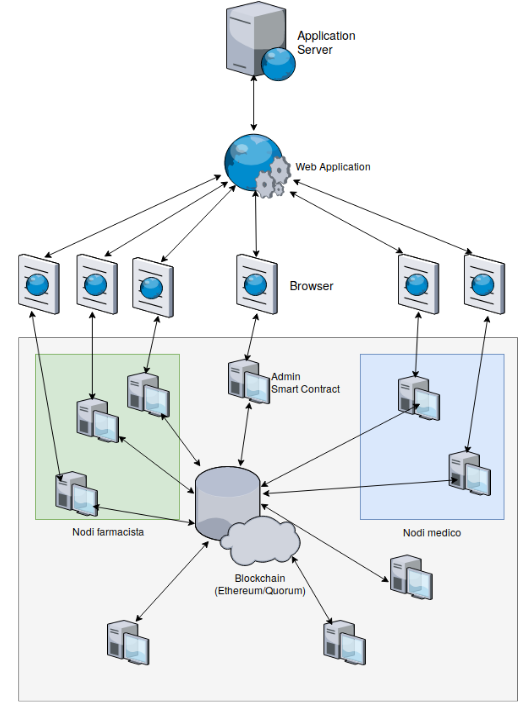
\includegraphics[width=.6\textwidth]{Implementazione/arch}
	%
	\caption{Diagramma del sistema}
	%
	\label{fig:diagramma del sistema}
	%
\end{figure}
%
Per gestire la prescrizione e l'erogazione delle ricette dematerializzate nonchè l'assegnazione dei ruoli all'interno della rete, la blockchain viene personalizzata mediante il deploy di uno specifico contratto di \textit{erogazione}, contenente la logica dell'applicazione. Gli utenti potranno interagire direttamente con la blockchain attraverso il proprio browser. L'applicazione decentralizzata è stata pensata come una \enquote*{single page application} con l'obiettivo di fornire una esperienza utente più fluida e simile alle applicazioni desktop dei sistemi operativi tradizionali. L'interfaccia è stata scritta utilizzando i linguaggi standard della programmazione web quali HTML5, CSS3 e JavaScript.
%
\section{Ricetta medica}
%
Il primo passo nell'implementazione dell'applicazione è stato quello di modellare l'oggetto "ricetta medica" secondo i requisiti enunciati. La ricetta medica dematerializzata si presenterà quindi in questo modo:
\begin{figure}[H]
	%
	\centering
	%
	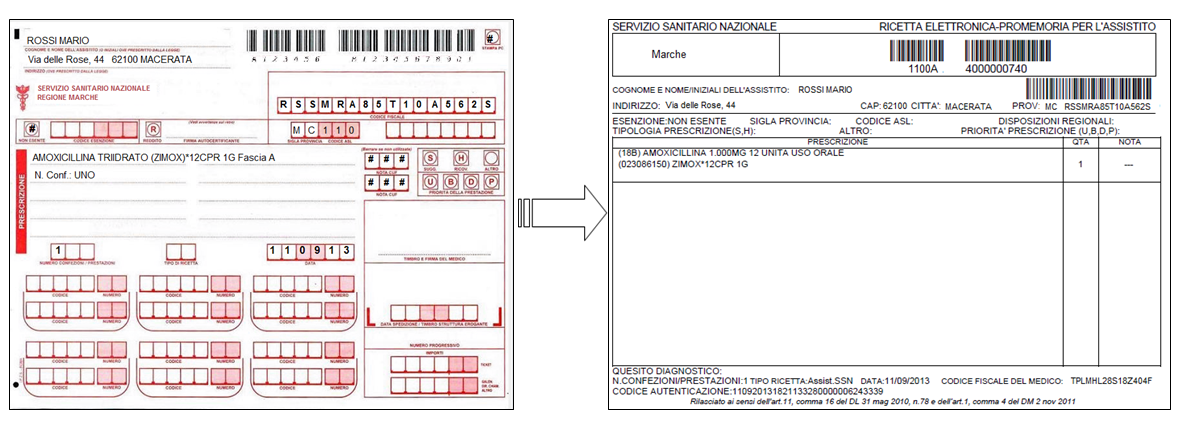
\includegraphics[width=.8\textwidth]{Implementazione/ricetta}
	%
	\caption{Struttura di una ricetta medica bianca dematerializzata}
	%
	\label{fig:struttura di una ricetta medica bianca dematerializzata}
	%
\end{figure}
ed è composta dai seguenti campi:
\begin{enumerate}
	\item \emph{NRE}. Codice univoco identificativo della ricetta dematerializzata. Viene utilizzato per ottimizzare la ricerca di una particolare ricetta all'interno della struttura dove vengono salvate.
	\item \emph{Timestamp}: rappresenta il timestamp preso all'atto della creazione della ricetta.
	\item \emph{Medico}: rappresenta il nome e il cognome del medico prescrittore.
	\item \emph{Paziente}: rappresenta il nome e il cognome del paziente.
	\item \emph{Prescrizione} rappresenta il contenuto della prescrizione.
	\item \emph{Qr-code}. Si è scelto di utilizzare il \gls{qrcode} come tecnologia per velocizzare l'erogazione della ricetta elettronica da parte dei farmacisti. Il farmacista andrà ad effettuare la scansione del qr-code per avviare il processo di erogazione della ricetta.
	\item \emph{Account Medico}: rappresenta l'indirizzo dell' account del medico prescrittore.
\end{enumerate}
Una volta ottenuta l'astrazione riguardante l'oggetto \enquote*{ricetta medica}, si è passati alla progettazione del contratto che regolasse la logica di funzionamento dell'applicazione sulla blockchain Quorum.
%
\section{Il contratto prescrizione}
%
La gestione della logica di funzionamento è stata realizzata mediante un contratto denominato \emph{Prescription.sol} caratterizzato dalle seguenti proprietà:
\begin{enumerate}
	\item una struttura per gestire i ruoli nel contratto (medico, farmacista e admin).
	\item una struttura per gestire le informazioni di un account. Nell'applicazione saranno composte per semplicità da nome, cognome e ruolo.
	\item una struttura per gestire le informazioni di una data ricetta. Nell'applicazione saranno composte da:
	      \begin{itemize}
	      	\item due variabili di tipo \emph{address}\footnote{Contiene un valore di 20 byte che corrisponde alla grandezza  indirizzo Ethereum} di cui una conterrà l'indirizzo sulla blockchain del medico prescrittore mentre l'altra onterrà l'indirizzo della farmacia che erogherà la farmacia. All'atto della creazione della ricetta questo dato particolare non è settato.
	      	\item una variabile di tipo \emph{bytes32} che conterrà il risultato dell'applicazione della primitiva crittografica \emph{Keccak-256 SHA3} sul contenuto della ricetta generata dal medico.
	      \end{itemize}
	\item per garantire invece che la modifica dello stato del contratto o l'invocazione delle funzioni del contratto vengano effettuate solo da determinati indirizzi, sono state inserite delle funzioni predefinite in Solidity denominate \emph{modifiers}. Ogni ruolo definito nel contratto ha la propria funzione modifiers associata in modo tale da poter garantire il corretto funzionamento del contratto. I modifiers vengono usate per modificare il corpo di una funzione e in particolare vengono preposti all'atto della chiamata della funzione per cui sono specificati. Il controllo ha successo solo se l'indirizzo che ha chiamato la funzione è del tipo giusto.
	\item il contratto infine contiene due strutture dati denominate \emph{mapping}. In Solidity un mapping  viene realizzato tramite la seguente sintassi $mapping (\textunderscore KeyType => \textunderscore ValueType) mapName$ dove \emph{\textunderscore KeyType} può essere la maggior parte dei tipo di dato\footnote{I tipi di dato non permessi come keyType sono mapping, array dinamici, struct ed enum} offerti in Solidity mentre \emph{\textunderscore ValueType} può essere qualsiasi tipo di dato. Questo tipo di dato può essere paragonato ad una tabella Hash. I due mapping sono stati definiti in accordo ai requisiti dell'applicazione in questo modo:
	      \begin{itemize}
	      	\item un mapping privato tra il codice univoco NRE e la struttura dati ricetta definita precedentemente. Questo mapping viene utilizzato per aumentare la velocità della ricerca della ricetta quando il farmacista procede ad effettuare il controllo su uno stato di una ricetta.
	      	\item un mapping privato tra l'indirizzo di un account sulla blockchain e la struttura contenente che gestisce le informazioni di un account.
	      \end{itemize}
	\item una serie di funzioni eseguibili che abilitano la logica del contratto. In particolare sono state implementate:
	      \begin{itemize}
	      	\item la funzione costruttrice del contratto che, all'atto del deploy sulla blockchain, setta l'account che effettua il deploy con il ruolo di amministratore. Si assume infatti che nella blockchain privata l'entità che procede al deploy del contratto sia l'entità di supervisione descritta nei capitoli precedenti.
	      	\item le funzioni per recuperare i dati anagrafici di un account.
	      	\item la funzione per recuperare il ruolo del mittente di una transazione.
	      	\item la funzione che permette di creare l'associazione tra nome, cognome, ruolo e indirizzo. A questa funzione viene associato il modifiers \emph{onlyAdmin}.
	      	\item la funzione per inserire una ricetta nella blockchain. Prende l'hash del contenuto della ricetta, l'nre associato e crea l'associazione con l'indirizzo che ha inviato la transazione che corrisponde al medico prescrittore. A questa funzione viene associato il modifiers \emph{onlyMedico}.
	      	\item la funzione che recupera una ricetta a partire dal NRE. Questa restituisce l'indirizzo del medico associato alla ricetta, il suo nre e l'hash. Nel caso in cui la ricetta non esiste nella blockchain verrà restituito il valore $0x0000000000000000000000000000000000000000$.
	      	\item la funzione che permette l'erogazione della ricetta da parte del farmacista. A partire dal NRE della ricetta va ad aggiornare il secondo campo address della ricetta inserendo l'indirizzo dell'account che l'ha appena erogata (quello della farmacia).
	      \end{itemize}
\end{enumerate}
%
\section{Creazione di una ricetta medica elettronica}
%
Abbiamo visto come, nella soluzione proposta, la ricetta dematerializzata viene concepita come un documento elettronico compilato dal medico prescrittore. Quest'ultimo infatti, tramite l'interfaccia specifica per il suo ruolo, andrà a riempire i campi della form corrispondenti alla ricetta elettronica. La pagina che viene presentata al medico è la seguente:
%
\begin{figure}[H]
	%
	\centering
	%
	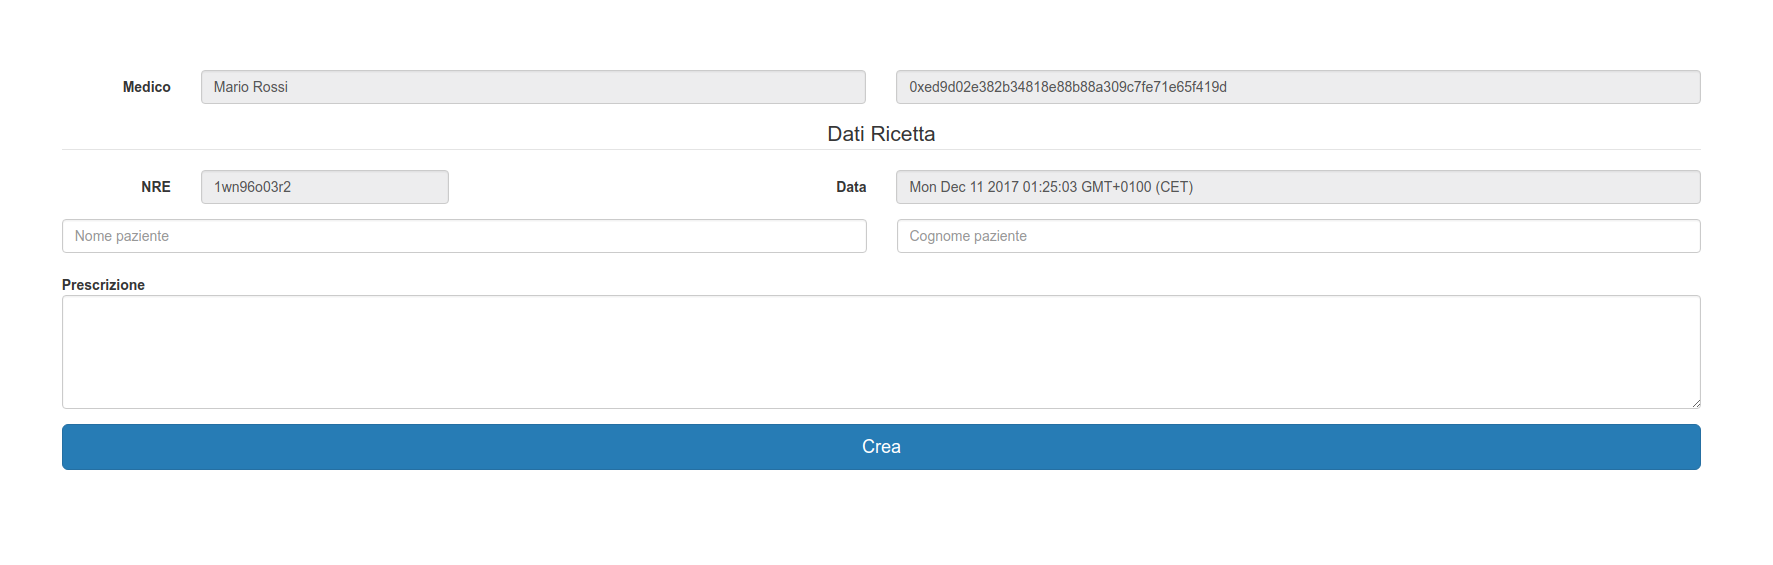
\includegraphics[width=1\textwidth]{Implementazione/prescrizione}
	%
	\caption{Schermata del medico prescrittore}
	%
	\label{fig:schermata del medico prescrittore}
	%
\end{figure}
%
Alcuni campi della form sono riempiti automaticamente e non possono essere modificati dal medico. In particolare le informazioni relative al nome e cognome del medico sono recuperate a partire dalla sessione di Web3.js attiva all'interno del browser (permette al browser di interagire direttamente con il contratto e la blockchain) mentre il timestamp viene generato lato client e il codice univoco NRE viene ricevuto dall'application server (tramite Express). La creazione di una ricetta elettronica da parte di un medico avviene nel modo seguente:
\begin{enumerate}
	\item All'atto del caricamento della pagina del medico, l'application server provvede a generare ed inviare un nuovo NRE al client.
	\item Il medico provvede a riempire i campi della form della ricetta elettronica.
	\item Una volta riempiti tutti i campi il medico provvede a creare la ricetta cliccando sul bottone \enquote*{crea}. Il submit della form avvierà la seguente sottoprocedura (il dialogo con la blockchain è asincrono):
	      \begin{enumerate}
	      	\item viene parsato il campo data al fine di renderlo adatto alla trasmissione.
	      	\item tutti i campi della ricetta vengono serializzati in un oggetto json. 
	      	\item l'oggetto json viene convertito in stringa per potervi applicare la primitiva crittografica sha3\footnote{Ethereum vuole una stringa come argomento da passare a questa api} messa a disposizione da Ethereum tramite le sue api. 
	      	\item a questo punto viene effettuata una transazione in quanto si va a chiamare la funzione del contratto che si occupa dell'inserimento di una ricetta sulla blockchain.
	      	\item una volta ottenuto il riscontro effettivo dell'avvenuto inserimento della ricetta sulla blockchain viene effettuata una chiamata post verso l'application server al quale viene passato lo stesso oggetto serializzato inviato sulla blockchain. 
	      	\item il server andrà prima a creare la struttura della ricetta elettronica (un documento in formato B6 landscape) inserendo tutti i campi come abbiamo visto nei paragrafi precedenti e, successivamente, andrà a creare il qr-code\footnote{Per la generazione del qr-code si è scelta una tra le tante librerire disponibili per Node. In questo caso \emph{qr-image}ancona17} contenente la stringa generata a partire dal json serializzato (così come è avvenuto nello step precedente) e lo inserirà all'interno della ricetta elettronica. Una volta generata la ricetta elettronica il server invierà il risultato al client permettendo al medico di salvare la ricetta elettronica oppure di creare una nuova ricetta. Si è scelto di dare la possibilità di stampa della ricetta dematerializzata (ripristinando così il promemoria essitente) per similitudine rispetto al sistema attuale tuttavia la scansione del qr-code può anche essere fatta tramite ricetta elettronica su smartphone permettendo così l'abbandono completo della carta nel processo di prescrizione delle ricette mediche.
	      \end{enumerate}
\end{enumerate}
Il procedimento appena descritto viene inoltre mostrato nel seguente diagramma delle sequenze:
%
\begin{figure}[H]
	%
	\centering
	%
	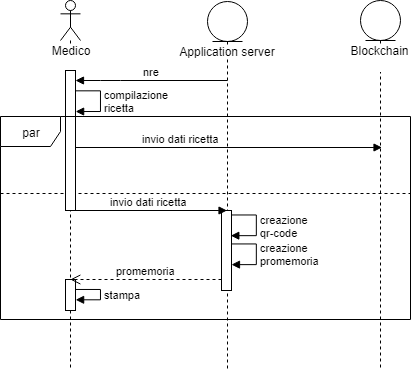
\includegraphics[width=.9\textwidth]{Implementazione/prescrizioneSeq}
	%
	\caption{Creazione di una ricetta dematerializzata}
	%
	\label{fig:creazione di una ricetta dematerializzata}
	%
\end{figure}
%
\section{Erogazione di una ricetta elettronica}
%
Una volta che la ricetta viene correttamente salvata sulla blockchain e viene generato il corretto promemoria elettronico (ed eventualmente stampato) per il paziente, quest'ultimo può recarsi in una farmacia per richiedere l'erogazione della prescrizione che ha appena ricevuto. Come avviene per il medico prescrittore anche per il farmacista è stata un'interfaccia esclusiva per il suo ruolo così fatta:
%
\begin{figure}[H]
	%
	\centering
	%
	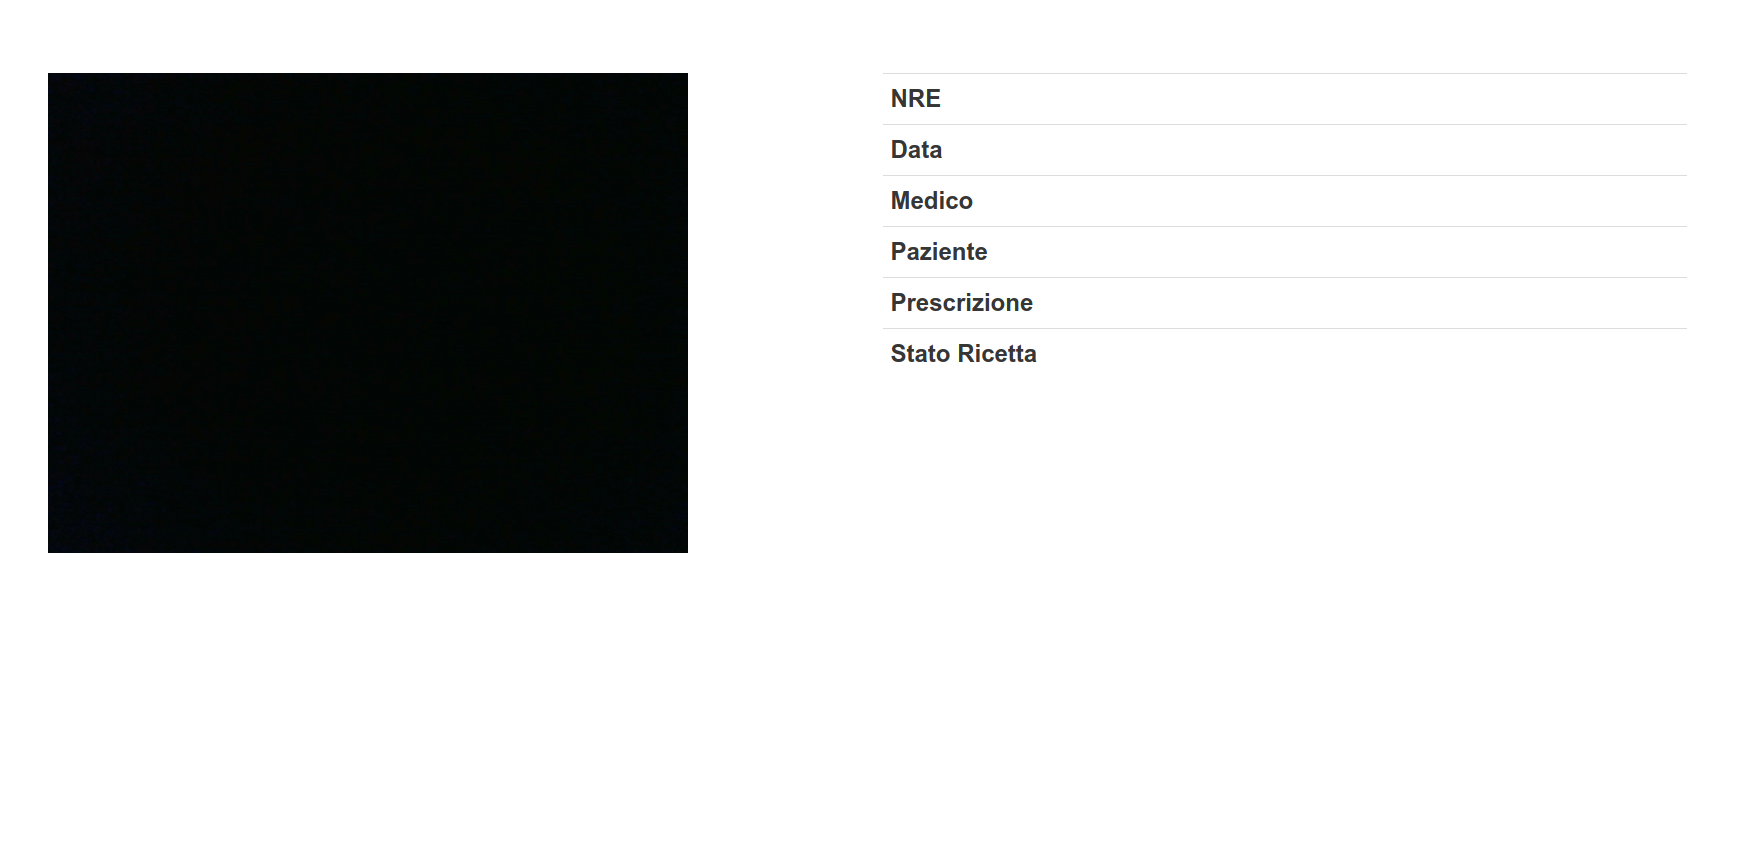
\includegraphics[width=1\textwidth]{Implementazione/farmacia}
	%
	\caption{Schermata del farmacista}
	%
	\label{fig:schermata del farmacista}
	%
\end{figure}
L'interfaccia è stata divisa in due zone:
\begin{itemize}
	\item Il box di sinistra andrà a contenere il feed della webcam. Sia per velocizzare la procedura di erogazione che per minimizzare l'errore dell'operatore (non è più necessario inserire i campi della ricetta manualmente per cercarla ed erogarla) è stato implementato uno scanner di codici qr-code che interagisce direttamente con la webcam del terminale dell'operatore. \\
	      Lo scanner di qr-code è stato implementato completamente mediante HTML5 (HTML5 compliant) per renderlo il più possibile compatibile con i browser attuali senza il bisogno di installare tecnologie abilitanti di terze parti (e.g. Flash player di Adobe).
	\item la griglia di destra invece viene automaticamente popolata all'atto della scansione del qr-code andando quindi a contenere il riassunto, mostrato a schermo, del contenuto della ricetta estratto dal codice appena scansionato.
\end{itemize}
L'erogazione di una ricetta da parte del farmacista avviene nel seguente modo:
\begin{enumerate}
	\item All'atto del caricamento della pagina del farmacista viene avviato lo scanner del qr-code e il suo feed sarà mostrato sull'interfaccia.
	\item Nel momento in cui si va a scansionare un codice qr-code contenuto sulla ricetta elettronica il client provvederà a parsare il contenuto del qrcode per popolare la griglia e preparare i dati per la ricerca della ricetta sulla blockchain.
	\item Una volta ottenuti tutti i campi della ricetta, il client ricrea la stringa che il client del medico prescrittore ha generato all'atto della creazione. Questo viene fatto perchè l'hash creato dal farmacista tramite i campi appena scansionati sarà confrontato con l'hash salvato dalla blockchain dal medico. Per far questo il client chiamerà la funzione del contratto addetta alla ricerca di una determinata ricetta medica passandogli il codice univoco NRE. La ricerca può avere due esiti diversi:
	      \begin{itemize}
	      	\item La ricetta non viene trovata. La funzione di ricerca restituisce valore $0x0000000000000000000000000000000000000000$ e il client notifica al farmacista che la ricetta che sta valutando non è valida in quanto non presente nella blockchain. Questo esito viene mostrato nella seguente figura:
	      	      %
	      	      \begin{figure}[H]
	      	      	%
	      	      	\centering
	      	      	%
	      	      	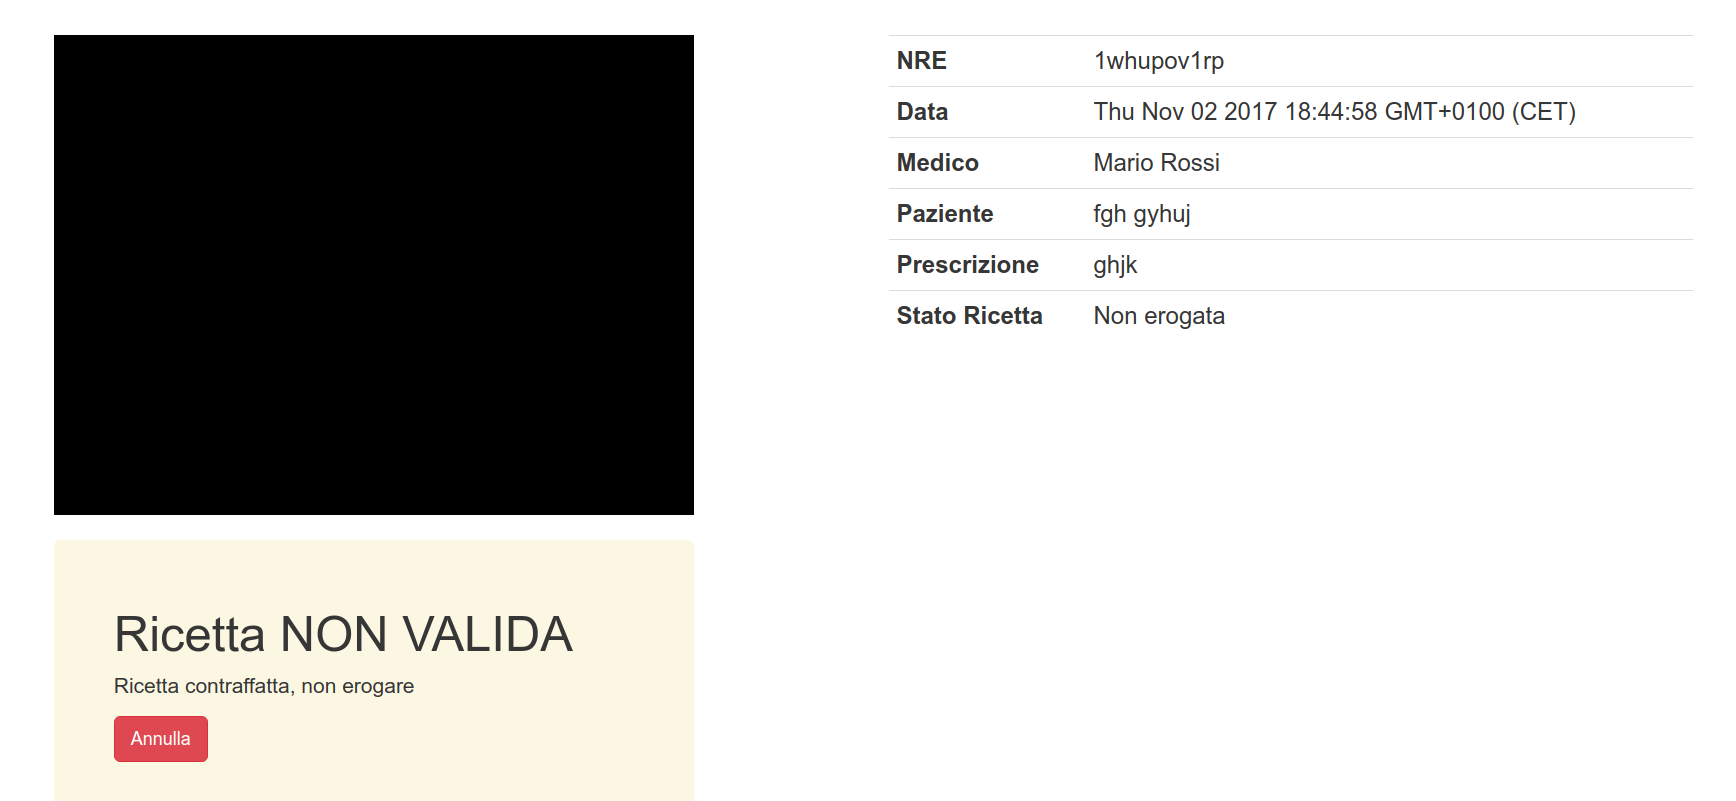
\includegraphics[width=.7\textwidth]{Implementazione/ricettaNO}
	      	      	%
	      	      	\caption{Ricetta medica non valida}
	      	      	%
	      	      	\label{fig:ricetta medica non valida}
	      	      	%
	      	      \end{figure}
	      	      %
	      	\item la ricetta viene trovata all'interno della blockchain e il risultato della transazione è un oggetto che contiene l'account del medico prescrittore, l'hash della ricetta e il suo stato(se è stata o meno già erogata). 	      
	      \end{itemize}
	\item L'hash della ricetta creato dal farmacista sarà ora confrontato con l'hash della ricetta ricevuto dalla blockchain come prova di integrità e non manomissione del contenuto della ricetta. I possibili risultati di questo confronto sono:
	      \begin{itemize}
	      	\item Ricetta valida. Il contenuto della ricetta corrisponde a quello salvato nella blockchain e non è già stata erogata. Il farmacista può procedere all'erogazione andando ad aggiornare lo stato della ricetta salvato sulla blockchain. Questa situazione viene mostrata nella seguente figura: 
	      	      %
	      	      \begin{figure}[H]
	      	      	%
	      	      	\centering
	      	      	%
	      	      	\includegraphics[width=.7\textwidth]{Implementazione/farmaciaOk}
	      	      	%
	      	      	\caption{Ricetta medica valida}
	      	      	%
	      	      	\label{fig:ricetta medica valida}
	      	      	%
	      	      \end{figure}
	      	      %
	      	\item La ricetta è valida ma è già stata erogata. Non è concessa la possibilità di erogare una seconda volta la ricetta elettronica. Questa situazione viene mostrata nella seguente figura: 
	      	      %
	      	      \begin{figure}[H]
	      	      	%
	      	      	\centering
	      	      	%
	      	      	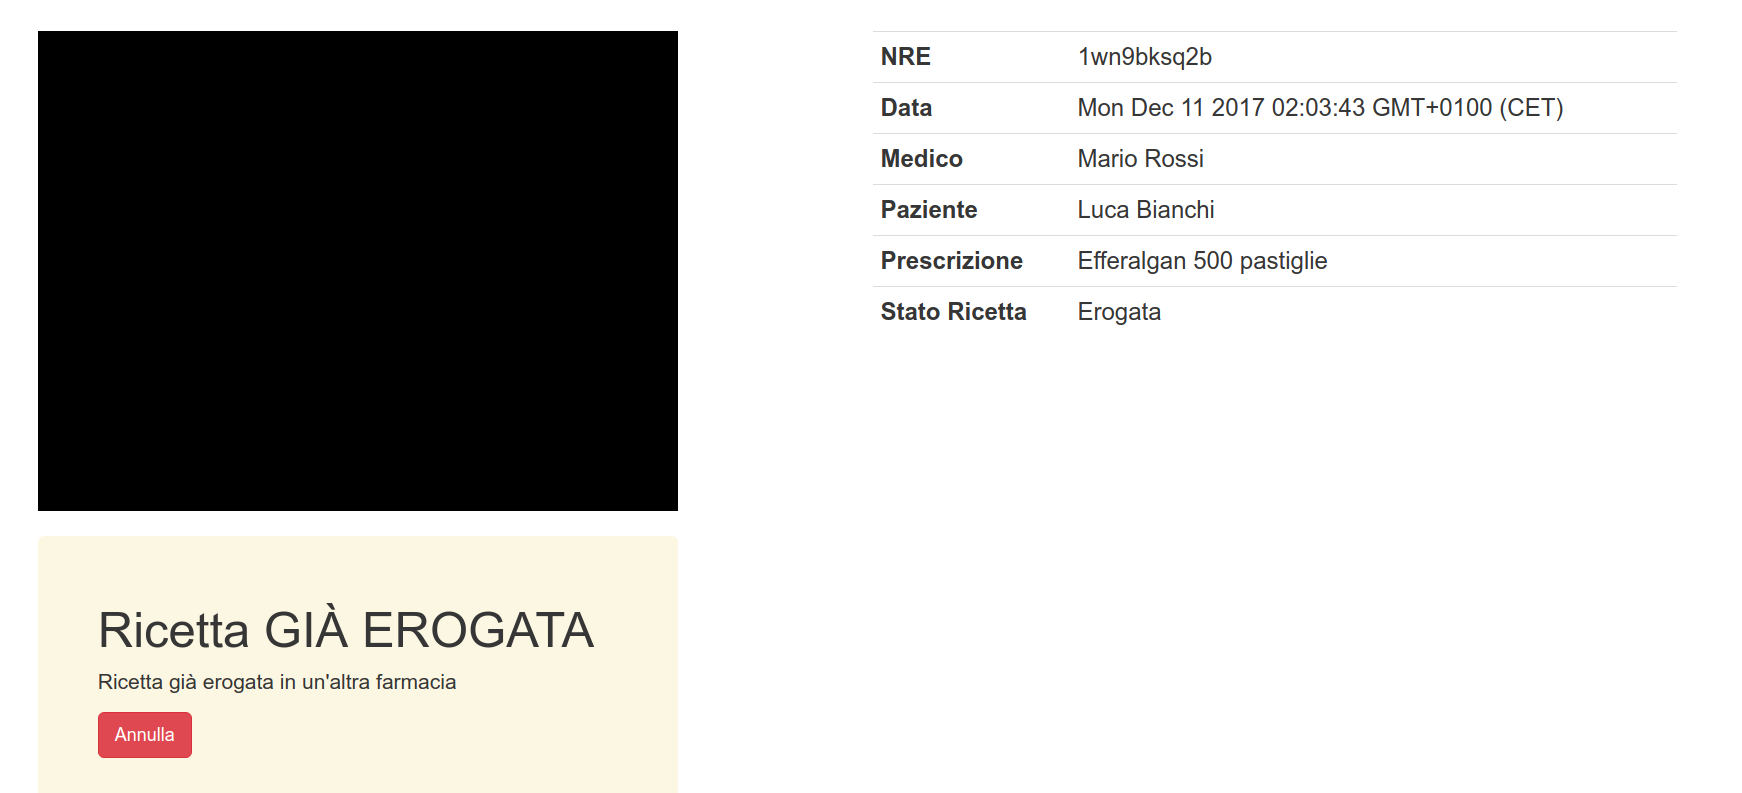
\includegraphics[width=.7\textwidth]{Implementazione/ricettaUSATA}
	      	      	%
	      	      	\caption{Ricetta medica già erogata}
	      	      	%
	      	      	\label{fig:ricetta medica già erogata}
	      	      	%
	      	      \end{figure}
	      	      %
	      	\item Ricetta medica non valida. Il contenuto della ricetta è stato alterato in qualche modo. L'erogazione viene rifiutata e la ricetta viene considerata non valida. Viene mostrata la stessa schermata di errore vista nel caso in cui la ricetta non viene trovata, ma con un codice di errore diverso.
	      \end{itemize}
\end{enumerate}
Il procedimento appena descritto viene inoltre mostrato nel seguente diagramma delle sequenze:
%
\begin{figure}[H]
	%
	\centering
	%
	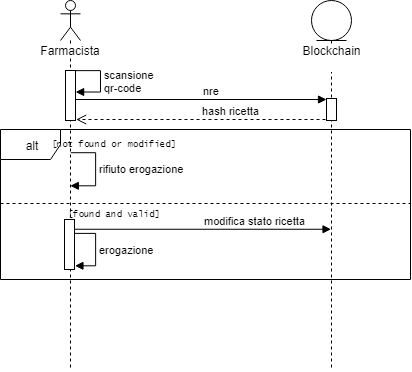
\includegraphics[width=.9\textwidth]{Implementazione/erogazioneSeq}
	%
	\caption{Creazione di una ricetta dematerializzata}
	%
	\label{fig:creazione di una ricetta dematerializzata}
	%
\end{figure}
%  	 
\section{Registrazione di nuovi account}
%
L'ammministratore presente all'interno della blockchain ha l'unico compito di gestire le associazioni tra gli indirizzi degli account presenti sulla catena e il ruolo che essi andranno a ricoprire nell'applicazione. La sua figura è stata inserita per avere una gestione più rapida del mapping account-ruolo, considerando anche il fatto che una figura di supervisione, seppur senza possibilità di fare altre azioni, sia necessaria in quanto stiamo parlando di un ambito sanitario nazionale La sua schermata è la seguente:
%
\begin{figure}[H]
	%
	\centering
	%
	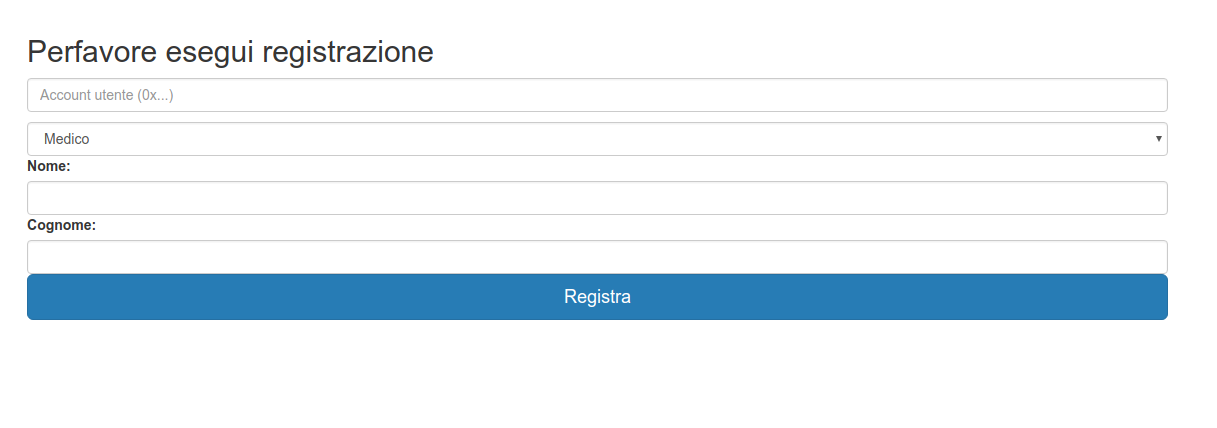
\includegraphics[width=.9\textwidth]{Implementazione/admin}
	%
	\caption{Assegnazione del ruolo da parte dell'amministratore}
	%
	\label{fig:assegnazione del ruolo da parte dell'amministratore}
	%
\end{figure}
% 
